\documentclass[tikz, varwidth=6in]{standalone}
\definecolor{ocra}{rgb}{1.0,0.9,0.7}

% arara: pdflatex: { interaction: batchmode }
% arara: latexmk: { clean: partial }
\begin{document}
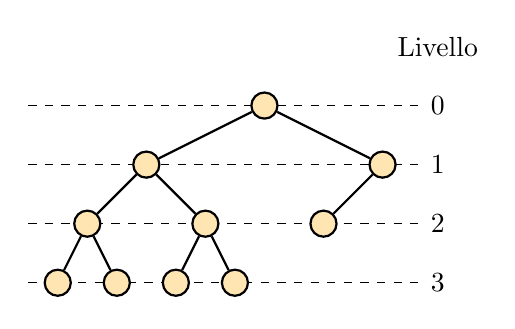
\begin{tikzpicture}[
	thick,
	level distance=0.75cm,
	level 1/.style={sibling distance=3cm},
	level 2/.style={sibling distance=1.5cm},
	level 3/.style={sibling distance=0.75cm}
]
\tikzset{
    treenode/.style = {circle, draw=black, align=center,fill=ocra},
}
\draw[dashed,thin] (-3,0) -- (2,0);
\draw[dashed,thin] (-3,-0.75) -- (2,-0.75);
\draw[dashed,thin] (-3,-1.5) -- (2,-1.5);
\draw[dashed,thin] (-3,-2.25) -- (2,-2.25);
\node at (2.2, 0.75) {Livello};
\node at (2.2, 0) {0};
\node at (2.2, -0.75) {1};
\node at (2.2, -1.5) {2};
\node at (2.2, -2.25) {3};

\node (A) [treenode] {}
	child { node[treenode] {}
		child { node[treenode] {}
			child { node[treenode] {} }
			child { node[treenode] {} }
		}
	child { node[treenode] {}
			child { node[treenode] {} }
			child { node[treenode] {} }
		}
	}
	child { node[treenode] {}
		child { node[treenode] {}	}
		child[missing] { node[treenode] {} }
	}
;
\end{tikzpicture}
\end{document}